\documentclass[12pt]{article}

\usepackage{hyperref}
\usepackage{graphicx}
\usepackage{longtable}
\usepackage{listings}
\usepackage[dvipsnames,table]{xcolor}

\lstdefinelanguage{SystemVerilog}%
  {morekeywords=[1]{module, endmodule, input, output, wire, logic, reg, always, begin, end, if, else, case, endcase, assign, parameter},
   morekeywords=[2]{logic, bit, int, enum, typedef},
   sensitive=true,
   morecomment=[l]{//},
   morecomment=[s]{/*}{*/},
   morestring=[b]",
  }

\lstset{
  language=SystemVerilog,
  basicstyle=\ttfamily\small,
  keywordstyle=[1]\color{blue}\bfseries,
  keywordstyle=[2]\color{purple},
  commentstyle=\color{gray}\itshape,
  stringstyle=\color{orange},
  breaklines=true,
  columns=fullflexible,
  frame=single,
  captionpos=b,
  showstringspaces=false
}

\graphicspath{{./img/}}

\definecolor{light-gray}{HTML}{E5E4E2}

\pagenumbering{arabic}

% VARIABLES
\def\UART_VERSION{v1.0.0}

\begin{document}
\begin{titlepage}
  \centering
  {\LARGE \textsc{Uart Implementation Reference}\par}
  {\vspace{1cm}}
  \UART_VERSION \\
  {\vspace{16cm}}
  Written by \\
  Kevin LASTRA
\end{titlepage}
\tableofcontents
\newpage

\section{Version}
\begin{tabular}{|p{1.5cm}|p{1.5cm}|p{2.5cm}|p{7cm}|}
  \hline
  \rowcolor{light-gray}\textbf{Version} & \textbf{Date} & \textbf{Author} & \textbf{Description} \\
  \hline
  v1.0.0 & 0 & Kevin Lastra & Initial release of the UART Implemenation Reference \\
  \hline
\end{tabular}
\newpage
\section{Introduction}
\subsection{Purpose of the manual}
The purpose of this manual is twofold. First, it serves as a 
comprehensive resource to document the Implementation of a 
Universal Asynchronous Receiver-Transmitter (UART). This process 
has been undertaken not only as a journey of self-learning but also 
as a way to share knowledge and contribute to the broader community
of developers, engineers, and enthusiasts.

\subsection{Audience}
This manual is primarly intended for design engineers who are 
involved in the development and implementation of communication
systems, particularly those working with embedded systems, 
microcontrollers, and hardware interfaces.

\newpage
\section{UART protocol overview}
The Universal Asynchronous Receiver-Transmitter (UART) is a 
fundamental hardware communication protocol used for asynchronous
serial communication. \\
This protocol is widely used in embedded systems, 
microcontrollers, and communication devices due to its simplicity and effectiveness
in handling relatively low-speed data transfer.
\subsection{UART fundamentals}
\subsubsection{Reception and transmission}
UART allows two devices to exchange data using only two wires, RX for receive data
and TX for transmit data.\\
\begin{figure}[h]
  \centering
  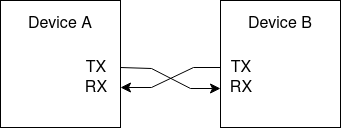
\includegraphics[width=0.6\textwidth]{UART_interface.png}
  \caption{Two UART's interfaces connected}
\end{figure}


\subsubsection{Asynchronous communication}
An asynchronous communication refers to a type of data transmission where the sender
and receiver do not rely on a shared clock signal for synchronization. Instead, each
device operates using its own internal clock and relies on specific timing 
conventions to ensure data is transmitted and received correctly. \\~\\
In asynchronous UART communication, the data is sent in discrete chunks 
(called data frames) over the communication channel, with the timing governed by 
agreed-upon parameters like baud rate and frame size.

\subsubsection{Baud rate}
The baud rate defines the speed at which data is transmitted over the communication
channel. It is usually expressed in bits per second (bps). \\
In the context of UART the baud rate specifies how many bits of data can be 
transmitted each second. Both transmitter and receiver must be set to the same baud
rate. \\~\\
The general formula for calculating the baud rate is:

\[Baud Rate = \frac{Clock Frequency}{Divisor}\]

\subsubsection{Data frame structure}
A UART data frame typically consists of: \\

\begin{table}[h]
  \centering
  \begin{tabular}{|p{3cm}|p{6cm}|p{3.5cm}|}
    \hline
    \rowcolor{light-gray}\textbf{Range name} & \textbf{Description} & \textbf{Implementation bit length} \\
    \hline
    Start bit & Signals the beginning of data transmission & 1 \\
    \hline
    Data bits & The actual data being sent & 5 - 9 \\
    \hline
    Parity & Used for error checking & 0 - 1 \\
    \hline
    Stop bit & Signals the end of the data transmission & 1 - 2 \\
    \hline
  \end{tabular}
\end{table}

\subsection{Advantages and limitations}
Advantages:
\begin{enumerate}
  \item Minimal pins required, essay to implement on a system.
  \item Low cost, because of its minimal hardware requirements the UART is a
        cost-effective solution.
  \item Widely supported.
  \item Simplicity in software implementation.
\end{enumerate}
limitations:
\begin{enumerate}
  \item Distance limitations, the maximum range depends on the baud rate, the quality
        of the wires and the environment (e.g. electromagnetic interferences).
  \item Relatively slow data transfer.
  \item Limited to two devices.
  \item Susceptibility to baud rate mismatch.
  \item Limited error detection, UART error detection is limited to parity checks and
        stop bits.
\end{enumerate}
\newpage
\section{Implementation}
\subsection{Design}
The UART implementation is composed of four primary modules: a Receiver, 
a Transmitter, a Clock Generator, and a control and status register with an 
AXI4 system interface.
\begin{figure}[h]
  \centering
  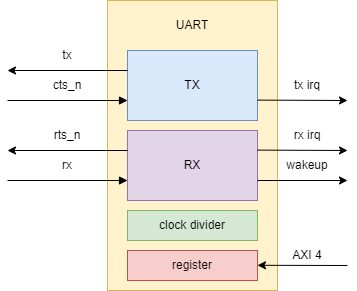
\includegraphics[scale=0.6]{UART_IMPL_DIAGRAM.png}
  \caption{Implementation diagram.}
\end{figure}

\subsubsection{Uart configuration}
The UART configuration register allows control over various operational 
aspects of the UART. It includes the following fields:
\begin{enumerate}
\item \textbf{flush\_rx / flush\_tx}: Used to clear the RX and TX asynchronous FIFOs, 
      respectively.
\item \textbf{flow\_control}: Enables or disables hardware flow control using the CTS\_N 
      (Clear To Send) and RTS\_N  (Request To Send) signals.
\item \textbf{parity}: Enables or disables parity checking and generation for data frames.
\item \textbf{master}: Defines which part of the UART (transmitter or receiver) is active. 
      This is only used in SIMPLEX or HALFDUPLEX communication, where only one direction is 
      active at a time.
\item \textbf{mode}: Specifies the UART communication mode:
      \begin{enumerate}
        \item \textbf{FULLDUPLEX}: Both transmitter and receiver are active and operate simultaneously. 
              This is the standard mode for most UART communication.
        \item \textbf{HALFDUPLEX}: Transmitter and receiver share the same communication line, but only 
              one can be active at a time. The master field determines which is currently active.
        \item \textbf{SIMPLEX}: Communication occurs in only one direction. The master field is used 
              to enable either TX or RX, but not both.
      \end{enumerate}
\end{enumerate}
This register is typically configured through the AXI4 interface during initialization or reconfiguration of the UART.
\subsubsection{Data frame}
The received and transmitted data frame is built has follows : \\

\noindent \begin{tabular}{|p{3cm}|p{3cm}|p{3cm}|p{3cm}|}
  \hline
  \rowcolor{light-gray}\textbf{Start} & \textbf{Data} & \textbf{Parity} & \textbf{Stop} \\
  \hline
  1 & 8 & *1  & 1 \\
  \hline
\end{tabular} \\~\\
\noindent (*) The parity bit is an optional feature.
\subsubsection{Receiver (RX)}
This module is responsible for sampling and decoding incoming serial data. It 
detects the start bit, samples each data bit based on the configured baud rate, 
check the parity bit (if enabled) and verifies the stop bit. Once a complete and valid frame 
is received, the data byte is stored in an asynchronous FIFO for further 
processing by the system. \\

\noindent The RX module provides a status register that reflects the current state of the receiver and 
any error conditions. The following bits are included:
\begin{enumerate}
\item \textbf{fifo\_empty}: Indicates that the RX FIFO is empty and no data is available to 
      read.
\item \textbf{fifo\_full}: Indicates that the RX FIFO is full and cannot accept more data.
\item \textbf{overrun\_error}: Set when new data arrives while the FIFO is full, meaning data 
      has been lost because the system did not read the previous data in time.
\item \textbf{parity\_error}: Set when parity checking is enabled and the received data has an 
      invalid or unexpected parity bit. This may also occur if parity is disabled but a 
      parity bit is present in the incoming frame.
\item \textbf{framing\_error}: Set when the received frame does not conform to the expected 
      UART format.
\end{enumerate}
These status bits can be used by the system to monitor the integrity and availability of received data and handle UART errors appropriately.

\subsubsection{Transmitter (TX)}
The transmitter handles the serialization of data from an asynchronous FIFO. 
It prepends a start bit, appends a parity bit and a stop bit, and transmits the 
bits sequentially according to the configured baud rate.

\noindent The transmitter module provides a status register that reports the current state 
of the TX FIFO and potential write errors. It includes the following bits:
\begin{enumerate}
\item \textbf{fifo\_empty}: Indicates that the TX FIFO is empty and no data is waiting to be 
      transmitted.
\item \textbf{fifo\_full}: Indicates that the TX FIFO is full and cannot accept additional 
      data.
\item \textbf{overrun\_error}: Set when the system writes new data to the TX FIFO while it 
      is already full. In this case, the new data is lost.
\end{enumerate}

\noindent These status bits help the system manage data transmission and ensure that write operations 
are performed safely and efficiently.

\subsubsection{Interrupts}
The UART module generates an interrupt when one or more bits in the status register are set 
and the corresponding bits in the interrupt mask are enabled. The interrupt signal remains 
active as long as at least one masked status condition is true.

\subsubsection{Wakeup line}
The wakeup signal is asserted by the RX module when it detects valid incoming serial data. 
The signal remains active for the duration of the reception, typically 8 to 9 clock cycles, 
corresponding to the length of a valid UART frame (start bit, data bits, optional parity, and 
stop bit). \\

\noindent This can be used to wake up the system from low-power modes when data activity is 
detected on the RX line.

\subsection{Control and status registers}

\noindent\begin{longtable}{|p{2.2cm}|p{1.4cm}|p{1.1cm}|p{1.1cm}|p{7cm}|}
    \hline
    \rowcolor{light-gray}\textbf{Register} & \textbf{Access type} & \textbf{Offset} & \textbf{Reset} & \textbf{Description} \\
    \hline
    \endhead
    \hline
    \endfoot
    divider & RW & 0x00 & 0x0 & Used to generate the UART clock by 
    dividing the system clock. \\
    \hline
    rx\_data & RO & 0x04 & 0x0 & Last received data. One-time read access. \\
    \hline
    rx\_status & RO & 0x08 & 0x0 & RX module status: \\
    & & & & \begin{tabular}{|c|c|}
              \hline
              \rowcolor{light-gray}Bit & Name \\
              \hline
              \rowcolor{white}
               0 & Fifo empty \\
               1 & Fifo full \\
               2 & Overrun error \\
               3 & Parity error \\
               4 & Framing error \\
              \hline
            \end{tabular} \\
    & & & & \\
    \hline
    rx\_irq\_mask & RW & 0x0C & 0x0 & Enables interrupts for specific bits in rx\_status \\
    \hline
    tx\_data & WO & 0x10 & 0x0 & Write data to TX asynchronous FIFO. If full overrun\_error 
    status will be set to 1. \\
    \hline
    tx\_status & RO & 0x14 & 0x0 & TX module status: \\
    & & & & \begin{tabular}{|c|c|}
              \hline
              \rowcolor{light-gray}Bit & Name \\
              \hline
              \rowcolor{white}
               0 & Fifo full \\
               1 & Fifo empty \\
               2 & Overflow error \\
              \hline
            \end{tabular} \\
    & & & & \\
    \hline
    tx\_irq\_mask & RO & 0x18 & 0x0 & Enables interrupts for specific bits in tx\_status \\
    \hline
    control & RW & 0x1C & 0x0 & Configure UART: \\
    & & & & \begin{tabular}{|c|l|}
              \hline
              \rowcolor{light-gray}\textbf{Bit} & \textbf{Name} \\
              \hline
              \rowcolor{white}
               0 & Flush tx FIFO \\
              \hline
               1 & Flush rx FIFO \\
              \hline
               2 & Enable/Disable flow control \\
              \hline
               3 & Enable/Disable parity bit  \\
              \hline
               4 & Master device. Used only \\ 
                 & on mode SIMPLEX or \\ 
                 & HALFDUPLEX. \\ 
                 & 1 - Use only TX line \\
                 & 0 - Use only RX line \\
              \hline
               [5:6] & Uart mode: \\ 
                     & 2'b00 : SIMPLEX \\
                     & 2'b01 : HALFDUPLEX \\
                     & 2'b20 : FULLDUPLEX \\
              \hline
            \end{tabular} \\
    & & & & \\
    \hline
    version & RO & 0x20 &  & Hold the current version implemented \\
    \hline
\end{longtable}

\subsection{Integration}
This section describes how to instantiate and integrate the UART module into other projects, 
including its parameters, ports, and interfaces.

\subsubsection{Parameters}
The module includes configurable parameters to adapt the UART to different system requirements:

\noindent \begin{tabular}{|p{4cm}|p{2cm}|p{7cm}|}
  \hline
  \rowcolor{light-gray}\textbf{Name} & \textbf{Length} & \textbf{Description} \\
  \hline
  REG\_ADDR\_MAP & 1 & Defines the base addresses of the UART internal registers for AXI4 access \\
  \hline
\end{tabular} \\~\\

\subsubsection{Inputs}
\noindent \begin{tabular}{|p{2cm}|p{2cm}|p{9cm}|}
  \hline
  \rowcolor{light-gray}\textbf{Name} & \textbf{Length} & \textbf{Description} \\
  \hline
  clk & 1 & System clock \\
  \hline
  rst\_n & 1 & Active-low reset signal \\
  \hline
  rx & 1 & Serial input line \\
  \hline
  cts\_n & 1 & Clear to send signal \\
  \hline
\end{tabular} \\~\\

\subsubsection{Outputs}
\noindent \begin{tabular}{|p{2cm}|p{2cm}|p{9cm}|}
  \hline
  \rowcolor{light-gray}\textbf{Name} & \textbf{Length} & \textbf{Description} \\
  \hline
  tx & 1 & Serial output line \\
  \hline
  rts\_n & 1 & Request to send signal \\
  \hline
  wakeup & 1 & Wakeup signal \\
  \hline
  rx\_irq & 1 & rx interrupt request \\
  \hline
  tx\_irq & 1 & tx interrupt request \\
  \hline
\end{tabular} \\~\\

\subsubsection{Interface}
\textbf{AXI4 Slave Interface}: Used to access the configuration and status registers.
\newpage
\subsubsection{Instantiation example}
\begin{lstlisting}[caption={UART Module Instantiation}]
  uart #(
    .REG_ADDR_MAP(0x5000_0000)
  ) uart_inst (
    .clk(clk),
    .rst_n(rst_n),
    .rx(rx_line),
    .tx(tx_line),
    .rts_n(rts_n_line),
    .cts_n(cts_n_line),
    .wakeup(uart_wakeup),
    .rx_irq(uart_irq),
    .tx_irq(uart_irq),
    .bus(axi4)
  );
  \end{lstlisting}

\section{Synthesis Corners}

\noindent \begin{tabular}{|p{2cm}|p{2cm}|p{9cm}|}
  \hline
  \rowcolor{light-gray}\textbf{Metric} & \textbf{Value} & \textbf{Conditions} \\
  \hline
  FMAX & X & X \\
  \hline
  LUTs & X & X \\
  \hline
  FFs & X & X \\
  \hline
  BRAMs & X & X \\
  \hline
\end{tabular} \\~\\

\end{document}